\begin{figure}[H]
\centering
\resizebox{0.7\textwidth}{!}{%
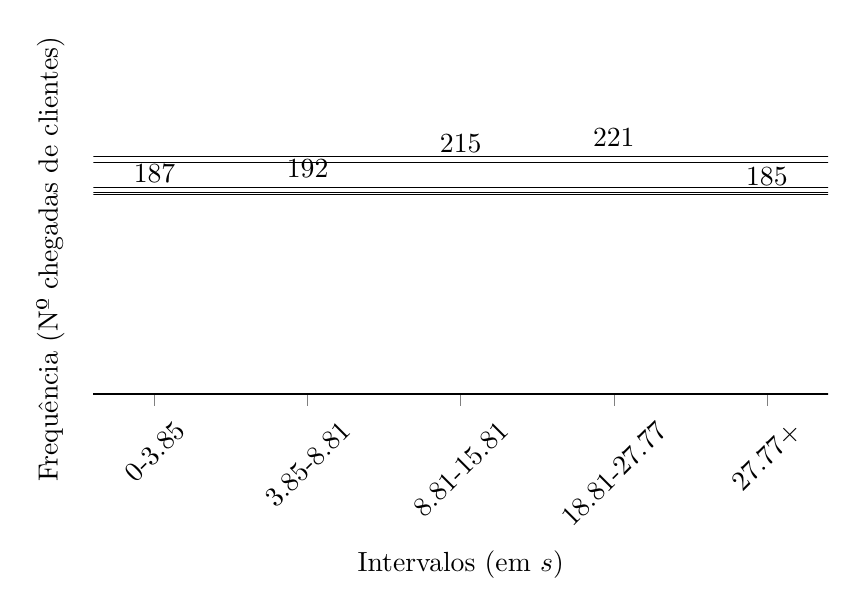
\begin{tikzpicture}

\begin{axis}[
    compat=newest, %Better label placement
    legend style={at={(0.5,-0.15)},
    anchor=north,legend columns=0},
    xtick={1,2,3,4,5,6},
    xticklabels={{$0$-$3.85$},
		         {$3.85$-$8.81$},
				 {$8.81$-$15.81$},
			     {$18.81$-$27.77$},
				 {$27.77$+}},
    xtick={1,...,10},
    nodes near coords,
    axis lines*=left,
    y axis line style={opacity=0},
    yticklabels={\empty},
    ytick style={draw=none},
     ymin=0, ymax=250,
    minor y tick num = 2,
    area style,
    height=5 cm,
    width=5cm,
    x tick label style={rotate=45},
    ybar=0pt,
    bar shift=0pt,
    bar width=32,
    width=0.9\textwidth,
      xlabel={Intervalos (em $s$)},
      ylabel={Frequ\^{e}ncia (Nº chegadas de clientes)}
    ]
    \addplot+[black, fill=white, ybar] plot coordinates {
        (1, 187) (2, 192) (3, 215) (4, 221)
	(5, 185)};
    

\end{axis}
\end{tikzpicture}
}%
\caption{Histograma da frequências da chegadas dos clientes por intervalos}
\label{p1:fig:grafico1}
\end{figure}

